%compile then compile with biber (for the biblio) then recompile
\documentclass[12pt]{article}

\usepackage{a4wide} % increase the typeset area
\usepackage{bm}
\usepackage{amsmath,amssymb}
\usepackage{enumitem}
\usepackage{graphicx}
\usepackage{color}
\usepackage{float} %to place figure H
\usepackage{multirow} %multirow for table
%\usepackage[super]{natbib} %exponant biblio
\usepackage{fourier} %for danger sign
\usepackage{chngcntr}
\usepackage{pifont} %for more symbol in enumerate

% Useful packages for table

\usepackage{array,multirow,makecell}
%\usepackage[linesnumbered]{algorithm2e}
\usepackage[table]{xcolor}
\setcellgapes{1pt}
\makegapedcells
\newcolumntype{R}[1]{>{\raggedleft\arraybackslash }b{#1}}
\newcolumntype{L}[1]{>{\raggedright\arraybackslash }b{#1}}
\newcolumntype{C}[1]{>{\centering\arraybackslash }b{#1}}



%hyperref
\usepackage[colorlinks]{hyperref}
\hypersetup{
	colorlinks=true,
	linkcolor=blue,
	filecolor=magenta,      
	urlcolor=blue,
	citecolor=blue
}

% captions
\usepackage{caption}
\newcommand{\vect}[1]{\hat{\boldsymbol{#1}}}
\usepackage{subcaption}
\counterwithin{figure}{section}
\makeatletter
\usepackage[labelformat=simple]{subcaption}
\newcommand\captionsubfigure{%
	\renewcommand\p@subfigure{}
	\renewcommand\thesubfigure{\thefigure.\alph{subfigure}}
}
\makeatother

%to make the appendix
\usepackage{appendix}

%code
\usepackage{listings}
\definecolor{backcolor}{RGB}{240, 240, 240}
\lstdefinestyle{bash}{
	commentstyle=\color{green},
	morecomment=[l][\color{magenta}]{\#},
	backgroundcolor=\color{backcolor},  
	breakatwhitespace=false,
	keepspaces=true,                        
	showspaces=false,                
	showstringspaces=false,
	showtabs=false,                  
	tabsize=1    
}

%%for footnote
%\usepackage[symbol]{footmisc}
%\renewcommand{\thefootnote}{\fnsymbol{footnote}}

%bibliography (with section)
\usepackage[backend=biber,style=numeric,sorting=nyt]{biblatex}
%\usepackage{biblatex} 
\addbibresource{biblio.bib}


% Titlepage
\newcommand{\reporttitle}{Internship Report : Innovative non-conformal finite element methods for augmented surgery}
\newcommand{\reportauthorOne}{Frédérique Lecourtier}
\newcommand{\reportsupervisorOne}{Michel Duprez}
\newcommand{\reportsupervisorTwo}{Emmanuel Franck}
\newcommand{\reportsupervisorThree}{Vanessa Lleras}
\newcommand{\reporttype}{Coursework}

%Algorithm
\usepackage{xcolor}
\usepackage[linesnumbered,noline,boxed,commentsnumbered]{algorithm2e}
%\usepackage[noline, linesnumbered]{algorithm2e}% http://ctan.org/pkg/algorithm2e
\SetNlSty{bfseries}{\color{black}}{}

% pour rajouter des commentaires en rouge !
\newcommand{\tmcolor}[2]{{\color{#1}{#2}}}
\newcommand{\modif}[1]{\tmcolor{red}{#1}}
\newcommand{\trad}[1]{\tmcolor{blue}{#1}}

\usepackage{amsthm}
\newtheorem*{Rem}{\textit{Remark}}
\newtheorem{Prop}{Proposition}[section]
\newtheorem{Def}{Definition}[section]
\newtheorem*{Example}{Example}

\setlength\parindent{0pt}

\usepackage{titlesec}
\setcounter{secnumdepth}{4}
\titleformat{\paragraph}
{\normalfont\normalsize\bfseries}{\theparagraph}{1em}{}
\titlespacing*{\paragraph}
{0pt}{3.25ex plus 1ex minus .2ex}{1.5ex plus .2ex}

\usepackage{fontawesome5}

\sloppy

\newcommand\numberthis{\addtocounter{equation}{1}\tag{\theequation}}

\allowdisplaybreaks

\begin{document}
	\nocite{*}
	
	\begin{titlepage}

\newcommand{\HRule}{\rule{\linewidth}{0.5mm}}

\begin{center}
	
\includegraphics[width = 0.5\linewidth]{images/logo-mimesis.png} \\ [1.5cm] 

	\textsc{\Large University of Strasbourg}\\[0.5cm] 
	\textsc{\large Master CSMI}\\[0.95cm] 
	
	\HRule \\[0.4cm]
	\huge\bfseries\reporttitle\par % Title of your document
	\HRule \\[0.4cm]
\end{center}

\vspace{1cm}

\begin{flushleft} \large
	\begin{minipage}{0.4\hsize}
		\textit{Authors:}\\
		\reportauthorOne
	\end{minipage} \hfill 
	\begin{minipage}{0.4\hsize}
		\textit{Supervisors:}\\
		\reportsupervisorOne\\
		\reportsupervisorTwo
	\end{minipage}
\end{flushleft}
\vspace{3 cm}
\makeatletter
Date: \@date
\hfill

\includegraphics[width = 0.2\linewidth]{images/inria.png}\\[1.5cm] 

\vfill % Fill the rest of the page with whitespace



\makeatother


\end{titlepage}


	\tableofcontents

	\newpage
	\section{Introduction}

This end of study internship is a 2nd year internship in the CSMI Master ("Calcul Scientifique et Mathématiques de l'Information") of the University of Strasbourg. It is the continuation of a project done during the first semester of M2, the main objective of this project was the discovery of an innovative non-conformal finite element method for augmented surgery, the $\phi$-FEM method. The purpose of this project was to have Cemosis and Mimesis collaborate through the use of Feel++ software (developed by Cemosis) in the framework of the $\phi$-FEM method (one of the research topics of the Mimesis team). This project was followed by a 6-month internship whose main objective was to correct the output of a Fourier Neural Operator (FNO) by a solver using the $\phi$-FEM method.

\subsection{Scientific Context}

Finite element methods (FEM) are used to solve partial differential equations numerically. These can, for example, represent analytically the dynamic behavior of certain physical systems (mechanical, thermodynamic, acoustic, etc.). Among other things, it is a discrete algorithm for determining the approximate solution of a partial differential equation (PDE) on a compact domain with boundary conditions. 

The standard FEM method, which requires precise meshing of the domain under consideration and, in particular, fitting with its boundary, has its limitations. In particular, in the medical field, meshing complex and evolving geometries such as organs (e.g. the liver) can be very costly. More specifically, in the application context of creating real-time digital twins of an organ, the standard FEM method would require complete remeshing of the organ each time it is deformed, which in practice is not workable. 

This is why other methods, known as non-conformal finite element methods, have emerged in the last few years. These include CutFEM \cite{burman_cutfem_2015} or XFEM \cite{moes_x-fem_2002}, based on the idea of introducing a fictitious domain larger than the domain under consideration. We're interested here in another non-conformal method, which we'll present in more detail later, called $\phi$-FEM. We'll only use it in the context of Poisson problem solving, for Dirichlet boundary conditions \cite{duprez_phi-fem_2020}. But the method has been extended to Neumann conditions \cite{duprez_new_2023} and then to solve various mechanical problems, including linear elasticity \cite[Chapter~2]{cotin_phi-fem_nodate} and heat transfer problems \cite[Chapter~5]{cotin_phi-fem_nodate}.

\subsection{Presentation of the team}

Created in January 2021 within ICube laboratory at the University of Strasbourg, \href{https://mlms.icube.unistra.fr/en/index.php/Presentation}{MLMS} ("Machine Learning, Modélisation et Simulation") team is interested in data, models and simulations for medical science and human motion. It brings together computer scientists, mathematicians, bio-mechanicians, and neuroscientists to develop functional, physical, and geometric models around a transverse axis "Assistance to medical interventions by computer". MLMS hosts the \href{https://mimesis.inria.fr/}{MIMESIS} project-team as a sub-team. The MIMESIS research team aims at creating real-time digital twins of an organ, with main application domains as surgical training and surgical guidance during complex interventions. In 2023, a new inria team NECTARINE will be created within MLMS, who will focus on scientific challenges related to neuro-stimulation in the clinical context. 

MIMESIS, directed by Stéphane Cotin, is a joint \href{https://www.inria.fr/fr}{Inria} ("Institut national de recherche en sciences et technologies du numérique") and \href{https://www.cnrs.fr/fr}{CNRS} ("Centre national de la recherche scientifique") Research Team. The Mimesis research team is working on a set of scientific challenges in scientific computing, data assimilation, machine learning and control, with the goal of creating real-time digital twins of an organ.

\subsection{Objectives}

The main objective of the internship was to combine finite element methods and Machine Learning in order to solve the Poisson problem with Dirichlet condition. More precisely, we want to train a neural network called Fourier Neural Network (FNO) \cite{li_fourier_2021} to predict the solutions of a PDE for a given problem family (i.e. a "type" of source term). This neural network is trained with a data set consisting of the $\phi$-FEM solutions of the problems considered. The predictions of this neural network will then be fed back into a finite element solver to apply a correction to improve the accuracy of the solution : this was the subject covered during the internship. The finite element methods considered will be presented in Section \ref{FEMs} and the FNO in Section \ref{FNO}.

It is important to note that the $\phi$-FEM method has an advantage that is very interesting in the context of organ geometries. Indeed, this type of geometry can deform in time and meshing a fictitious domain around this geometry avoids having to remesh the geometry in time. Thus only the levelset function will be modified and the mesh can be fixed. Moreover, a Cartesian mesh of the fictitious domain allows us to use the same type of neural network as those applied to images (especially FNO).

To be more precise, we will test different correction methods (presented in Section \ref{Corr.methods}) on different problems (presented in Section \ref{Corr.problems}) which will enable us to use the network prediction to help the solver get as close as possible to the solution. We will start by testing these different types of solver on an analytical solution (Section \ref{Corr.results.ana}), then on a "manually perturbed" solution (Section \ref{Corr.results.disturbed}) and finally on a $\phi$-FEM solution (Section \ref{Corr.results.phifem}).

After testing the various types of correction on the previous test cases, we'll apply these same methods to the prediction of an FNO (Section \ref{Corr.results.FNO}). The main objective is to enable the combination of FNO and correction to be more accurate than the conventional $\phi$-FEM solver. By first testing the different corrections on the previous test cases, we hope to get an idea of the order of errors to be expected. During the course of the internship, we realized that the results obtained on the FNO did not correspond to the expected analytical results. For this reason, other types of neural networks were considered, namely multi-perceptron networks (Section \ref{Corr.results.neural_net.multiperceptron}) and PINNs (Section \ref{Corr.results.neural_net.PINNs}), with the aim of checking whether the results obtained are related to the use of the FNO.

\subsection{Deliverables}

In the context of the internship, the following deliverables are provided:

\begin{enumerate}[label=\textbullet]
	\item a \href{https://github.com/flecourtier/phifem_stage/blob/main/docs/suivi/suivi.pdf}{weekly tracking report}, written in French, was produced as the internship progressed, listing the objectives and results for each week.
	\item a \href{https://github.com/flecourtier/phifem_stage}{github repository} containing all the code allowing to reproduce the results presented in this report, as well as the documents written during the internship. \modif{ajouter les codes en ligne}
	\item an \href{https://flecourtier.github.io/phifem_stage/phifem_project/1.0.3/main_page.html}{online report} generated with a tool called \href{https://antora.org/}{antora}. A continuous integration has been set up on github to execute a python code for each new push, enabling the latex file to be converted directly into this antora documentation.
	\item \modif{a code documentation has also been set up with sphinx.} %https://www.sphinx-doc.org/en/master/
\end{enumerate}
	
	\newpage
	\section{Finite Element Methods (FEMs)}
\graphicspath{{images/FEM}}

In the following, we will consider the Poisson problem with Dirichlet condition (homogeneous or inhomogeneous):

\textbf{Problem :} Find $u : \Omega \rightarrow \mathbb{R}^d$ such that

\begin{equation*}
	\left\{
		\begin{aligned}
			-\Delta u &= f \; &&\text{in } \; \Omega \\
			u&=g \; &&\text{on } \; \partial\Omega
		\end{aligned}
	\right.
\end{equation*}

with $\Delta$ the Laplace operator and $\Omega\subset\mathbb{R}^d$ a lipschitzian bounded open set (and $\partial\Omega$ its boundary).

\textbf{Associated physical model :} Newtonian gravity, Electrostatics, Fluid dynamics...

\subsection{Standard FEM}

\subsubsection{Some notions of functional analysis.}

\modif{AJOUTER : Déf Espace de Hilbert (+ ce qu'il faut pour def ça : Espace de Soboloev ? ... ) + Déf $L^2$,}

\subsubsection{General principle of the method}

Let's consider a domain $\Omega$ whose boundary is denoted $\partial\Omega$. We seek to determine a function $u$ defined on $\Omega$, solution of a partial differential equation (PDE) for given boundary conditions.

The general approach of the finite element method is to write down the variational formulation of this PDE, thus giving us a problem of the following type:

\textbf{Variational Problem :}
\begin{equation*}
	\text{Find } u\in V \text{ such that } a(u,v)=l(v), \;\forall v\in V
\end{equation*}

where $V$ is a Hilbert space, $a$ is a bilinear form and $l$ is a linear form.

To do this, we multiply the PDE by a test function $v\in V$, then integrate over $L^2(\Omega)$.

The idea of FEM is to use Galerkin's method. We then look for an approximate solution $u_h$ in $V_h$, a finite-dimensional space dependent on a positive parameter $h$ such that

\begin{equation*}
	V_h\subset V, \quad \dim V_h = N_h<\infty, \quad \forall h>0
\end{equation*}

The variational problem can then be approached by :

\textbf{Approach Problem :}
\begin{equation*}
	\text{Find } u_h\in V_h \text{ such that } a(u_h,v_h)=l(v_h), \;\forall v_h\in V
\end{equation*}

As $V_h$ is of finite dimension, we can consider a basis $(\varphi_1,\dots,\varphi_{N_h})$ of $V_h$ and thus decompose $u_h$ on this basis as :

\begin{equation}
	\label{decomp1}
	u_h=\sum_{i=1}^{N_h}u_i\varphi_i	
\end{equation}

The approached problem is then rewritten as

\begin{equation*}
	\text{Find } u_1,\dots,u_{N_h} \text{ such that } \sum_{i=1}^{N_h}u_i a(\varphi_i,v_h)=l(v_h), \;\forall v_h\in V 
\end{equation*}

and

\begin{equation*}
	\text{Find } u_1,\dots,u_{N_h} \text{ such that } \sum_{i=1}^{N_h}u_i a(\varphi_i,\varphi_j)=l(\varphi_j), \;\forall j\in \{1,\dots,N_h\}
\end{equation*}

Solving the PDE involves solving the following linear system:
\begin{equation*}
	AU=b
\end{equation*}
with
\begin{equation*}
	A=(a(\varphi_i,\varphi_j))_{1\le i,j\le N_h}, \quad U=(u_i)_{1\le i\le N_h} \quad \text{and} \quad b=(l(\varphi_j))_{1\le j\le N_h}
\end{equation*}

\subsubsection{Some details on FEM}

\modif{Notions à aborder : ef de Lagrange + unisolvance + maillage + Transformation géométrique}

After having seen the general principle of FEM, it remains to define the $V_h$ spaces and the $\{\varphi_i\}$ basis functions.

\begin{Rem}
	The choice of $V_h$ space is fundamental to have an efficient method that gives a good approximation $u_h$ of $u$. In particular, the choice of the $\{\varphi_i\}$ basis of $V_h$ influences the structure of the $A$ matrix in terms of its sparsity and its condition number.
\end{Rem}

\paragraph{Finite Lagrange Element}

\trad{Le type le plus classique et le plus simple d'éléments finis sont les éléments finis de Lagrange.}

\begin{Def}[Lagrange Finite Element]
	\trad{Un élément fini de Lagrange est un triplet $(K,\Sigma,P)$ tel que 
	\begin{enumerate}[label=\textbullet]
		\item $K$ est un élément géométrique de $\mathbb{R}^n$ ($n=1,2$ ou $3$), compact, connexe et d'intérieur non vide.
		\item $\Sigma=\{a_1,\dots,a_N\}$ est un ensemble fini de $N$ points distincts de $K$.
		\item $P$ est un espace vectoriel de dimension finie de fonctions réelles définies sur $K$ et tel que $\Sigma$ soit $P$-unisolvant (donc $\dim P=N$).
	\end{enumerate}}
\end{Def}

\begin{Rem}
	\trad{On dit que $\Sigma$ est $P$-unisolvant si et seulement si pour tous réels $\alpha_1,\dots,\alpha_N$, il existe un unique élément $p$ de $P$ tel que $p(a_i)=\alpha_i,i=1,\dots,N$. 
	Ceci revient à dire que la fonction}
	\begin{align*}
		L \; : \; P &\rightarrow \mathbb{R}^N \\
		p &\mapsto(p(a_1),\dots,p(a_N))
	\end{align*}
	\trad{est bijective.}
\end{Rem}

\begin{Rem}
	En pratique, pour montrer que $\Sigma$ est $P$-unisolvant, on vérifiera simplement que $\dim P=card(\Sigma)$ puis on montrera l'injectivité ou la surjectivité de $L$. L'injectivité  de $L$ se démontre en établissant que la seule fonction de $P$ s'annulant sur tous les points de $\Sigma$ est la fonction nulle. La surjectivité de $L$ se démontre en exhibant une famille $p_1,\dots,p_N$ d'éléments de $P$ tels que $p_i(a_j)=\delta_{ij}$. En effet, étant donné des réels $\alpha_1,\dots,\alpha_N$, la fonction $p=\sum_{i=1}^N\alpha_i p_i$ vérifie alors $p(a_j)=\alpha_j,j=1\dots,N$. 
\end{Rem}

\modif{A mettre plus loin (base de $P_1$ à définir d'abord)}
\begin{Example}
	\trad{Soit $K$ le segment $[a_1,a_2]$. Montrons que $\Sigma=\{a_1,a_2\}$ est $P$-unisolvant pour $P=\mathbb{P}^1$. Comme $\{1,x\}$ est une base de $\mathbb{P}^1$, on a bien $\dim P = \text{card } \Sigma = 2$. 
		
	De plus, on peut écrire $p_i=\alpha_i x+\beta_i, i=1,2$. Ainsi
	\begin{equation*}
		\left\{\begin{aligned}
			&p_1(a_1)=1 \\
			&p_1(a_2)=0
		\end{aligned}\right. \quad \iff	\quad
		\left\{\begin{aligned}
			&\alpha_1 a_1+\beta_1=1 \\
			&\alpha_1 a_2+\beta_1=0
		\end{aligned}\right. \quad \iff \quad
		\left\{\begin{aligned}
		&\alpha_1 = \frac{1}{a_1-a_2} \\
		&\beta_1 = -\frac{a_2}{a_1-a_2}
	\end{aligned}\right.
	\end{equation*}
	et
	\begin{equation*}
		\left\{\begin{aligned}
			&p_2(a_1)=0 \\
			&p_2(a_2)=1
		\end{aligned}\right. \quad \iff	\quad
		\left\{\begin{aligned}
			&\alpha_2 a_1+\beta_2=0 \\
			&\alpha_2 a_2+\beta_2=1
		\end{aligned}\right. \quad \iff \quad
		\left\{\begin{aligned}
			&\alpha_1 = \frac{1}{a_2-a_1} \\
			&\beta_1 = -\frac{a_1}{a_2-a_1}
		\end{aligned}\right.
	\end{equation*}
	Donc
	\begin{equation*}
		p_1(x)=\frac{x-a_2}{a_1-a_2} \quad \text{and} \quad p_2(x)=\frac{x-a_1}{a_2-a_1}
	\end{equation*}
	On en déduit la surjectivité de $L$ et $\Sigma$ est $\mathbb{P}^1$-unisolvant.}
	\end{Example}

\paragraph{Mesh}

\trad{La première étape consiste à construire un maillage de $\Omega$.}

\begin{Rem}
	\trad{La partie de génération de maillage est une étape importante }
\end{Rem}

\subsubsection{Application to the Poisson problem}

\modif{Ajouter formulation variationnel Poisson}

\begin{Prop}[Lax-Milgram]
	
	Let $a$ be a continuous, coercive bilinear form on $V$ and $l$ a continuous, linear form on $V$. Then the variational problem has a unique solution $u\in V$. 
	
	Moreover, if the bilinear form is symmetrical, $u$ is a solution to the following minimization problem:
	\begin{equation*}
		J(u)=\min_{v\in V} J(v), \quad J(v)=\frac{1}{2}a(v,v)-l(v)
	\end{equation*}
\end{Prop}

It can then be shown that the Poisson problem with Dirichlet condition has a unique weak solution.

\modif{rajouter preuve}

\subsection{$\phi$-FEM}

\modif{TO COMPLETE !}

+test

%The Φ-FEM method has an advantage that is very interesting in the context of organ geometries. Indeed, this type of geometry can deform in time and meshing a fictitious domain around this geometry avoids having to remesh the geometry in time. Thus only the levelset function will be modified and the mesh can be fixed. Moreover, a Cartesian mesh of the fictitious domain allows us to use the same type of neural network as those applied to images: this is the subject that will be approached during the internship.


	
	\newpage	
	\section{Fourier Neural Operator (FNO)} \label{FNO}
\graphicspath{{images/fourier}}

\modif{Est-ce que je rajouter réseau multi-perceptron et PINNs ? Si oui section "Neural Networks" puis sous-sections FNO,MultiPerceptron,PINNs}

We will now introduce Fourier Neural Operators (FNO). For more information, please refer to the following article \cite{li_fourier_2021}. \modif{+ add article Killian}

In image treatment, we call image tensors of size $ni\times nj\times nk$, where $ni\times nj$ corresponds to the image resolution and $nk$ corresponds to its number of channels. For example, an RGB (Red Green Blue) image has $nk=3$ channels. 
We choose here to present the FNO as an operator acting on discrete images. Reference articles present it in its continuous aspect, which is an interesting point of view. Indeed, it is thanks to this property that it can be trained/evaluated with images of different resolutions.

The FNO methodology creates a relationship between two spaces from a finite collection of observed input-output pairs. \modif{Est-ce que je gardes cette phrase ?}

\modif{A rajouter : implémentation effectuée/fournie par Vincent Vigon + on ne trouvera pas ici de test de variation des paramètres (modes, width...)}

\subsection{Architecture of the FNO}

The following figure (Figure \ref{FNO_schema}) describes the FNO architecture in detail:

\begin{figure}[H]
	\includegraphics[width=\linewidth]{"fno_schema.png"}
	\captionof{figure}{Architecture of the FNO.}
	\label{FNO_schema}
\end{figure}

The architecture of the FNO is as follows:

\begin{equation*}
	G_\theta = Q \circ \mathcal{H}_\theta^L \circ \dots \circ \mathcal{H}_\theta^1 \circ P
\end{equation*}

\newpage

We'll now describe the composition of the Figure \ref{FNO_schema} in a little more detail :
\begin{enumerate}[label=\textbullet]
	\item We start with input X of shape (batch\_size, height, width, nb\_channels) with batch\_size the number of images to be processed at the same time, height and width the dimensions of the images and nb\_channels the number of channels. Simplify by (bs,ni,nj,nk).
	\item We perform a $P$ transformation in order to move to a space with more channels. This step enables the network to build a sufficiently rich representation of the data.  For example, a Dense layer (also known as fully-connected) can be used. 	
	\item We then apply $L$ Fourier layers, noted $\mathcal{H}_\theta^l,\; l=1,\dots,L$, whose specifications will be detailed in Section \ref{FNO.fourierlayer}.
	\item We then return to the target dimension by performing a $Q$ transformation. In our case, the number of output channels is 1.
	\item We then obtain the output of the $Y$ model of shape (bs,ni,nj,1). 
\end{enumerate}

\subsection{Fourier Layer structure} \label{FNO.fourierlayer}

Each Fourier layer is divided into two sublayers:

\begin{equation*}
	\tilde{Y}=\mathcal{H}_\theta^l(\tilde{X})=\sigma\left(\mathcal{C}_\theta^l(\tilde{X})+\mathcal{B}_\theta^l(\tilde{X})\right)
\end{equation*}

where
\begin{enumerate}[label=\textbullet]
	\item $\tilde{X}$ corresponds to the input of the current layer and $\tilde{Y}$ to the output.
	\item $\sigma$ is an activation function. For $l=1,\dots,L-1$, we'll take the activation function ReLU (Rectified Linear Unit) and for $l=L$ we'll take the activation function GELU (Gaussian Error Linear Units).
	\begin{figure}[H]
		\centering
		\includegraphics[width=0.3\linewidth]{"activation_functions.png"}
		\captionof{figure}{Activation functions used.}
	\end{figure}
	
	\item $\mathcal{C}_\theta^l$ is a convolution layer where convolution is performed by FFT (Fast Fourier Transform). For more details, see Section \ref{FNO.conv_sublayer}.
	\item $\mathcal{B}_\theta^l$ is the "bias-layer". For more details, see Section \ref{FNO.bias_sublayer}.
\end{enumerate}

\subsubsection{Convolution sublayer} \label{FNO.conv_sublayer}

Each $\mathcal{C}_\theta^l$ convolution layer contains a trainable kernel $\hat{W}$ and performs the transformation

\begin{equation*}
	\mathcal{C}_\theta^l(X)=\mathcal{F}^{-1}(\mathcal{F}(X)\cdot\hat{W})
\end{equation*}

where $\mathcal{F}$ corresponds to the 2D Discrete Fourier Transform (DFT) on a $ni\times nj$ resolution grid and
\begin{equation*}
	(Y\cdot\hat{W})_{ijk}=\sum_{k'}Y_{ijk'}\hat{W}_{ijk'}
\end{equation*}
In other words, this transormation is applied channel by channel.

\begin{Rem}
	An image is fundamentally a signal. Just as 1D signals show changes in amplitude (sound) over time, 2D signals show variations in intensity (light) over space. The Fourier transform allows us to move from the spatial or temporal domain into the frequency domain. In a sound signal (1D signal), low frequencies represent low-pitched sounds and high frequencies represent high-pitched sounds. In the case of an image (2D signal), low frequencies represent large homogeneous surfaces and blurred parts, while high frequencies represent contours, more generally abrupt changes in intensity and, finally, noise.
\end{Rem}

The 2D DFT is defined by :

\begin{equation*}
\mathcal{F}(X)_{ijk}=\frac{1}{ni}\frac{1}{nj}\sum_{i'=0}^{ni-1}\sum_{j'=0}^{nj-1}X_{i'j'k}e^{-2\sqrt{-1}\pi\left(\frac{ii'}{ni}+\frac{jj'}{nj}\right)}
\end{equation*}

The inverse of the 2D DFT is defined by :

\begin{equation*}
\mathcal{F}^{-1}(X)_{ijk}=\sum_{i'=0}^{ni-1}\sum_{j'=0}^{nj-1}X_{i'j'k}e^{2\sqrt{-1}\pi\left(\frac{ii'}{ni}+\frac{jj'}{nj}\right)}
\end{equation*}

We can easily show that $\mathcal{F}$ is the reciprocal function of $\mathcal{F}^{-1}$. We have 

\begin{align*}
	\mathcal{F}^{-1}(\mathcal{F}(X))_{ijk}&=\sum_{i'=0}^{ni-1}\sum_{j'=0}^{nj-1}\mathcal{F}(X)_{i'j'k}e^{2\sqrt{-1}\pi\left(\frac{ii'}{ni}+\frac{jj'}{nj}\right)} \\	
	&=\frac{1}{ni}\frac{1}{nj}\sum_{i'j'}\sum_{i''j''}X_{i''j''k}e^{-2\sqrt{-1}\pi\left(\frac{i'i''}{ni}+\frac{j'j''}{nj}\right)}e^{2\sqrt{-1}\pi\left(\frac{ii'}{ni}+\frac{jj'}{nj}\right)} \\
	&=\frac{1}{ni}\frac{1}{nj}\sum_{i''j''}X_{i''j''k}\sum_{i'j'}e^{2\sqrt{-1}\pi\frac{i'}{ni}(i-i'')}e^{2\sqrt{-1}\pi\frac{j'}{nj}(j-j'')}
\end{align*}

Let

\begin{equation*}
	S=\sum_{i'j'}e^{2\sqrt{-1}\pi\frac{i'}{ni}(i-i'')}e^{2\sqrt{-1}\pi\frac{j'}{nj}(j-j'')}
\end{equation*}

Thus
\begin{enumerate}[label=\textbullet]
	\item If $(i,j)=(i'',j'')$ : $S=\sum_{i',j'}1=ni\times nj$
	\item If $(i,j)\ne(i'',j'')$ : 
	\begin{align*}
		S&=\sum_{i'}\left(e^{\frac{2\sqrt{-1}\pi}{ni}(i-i'')}\right)^{i'}\sum_{j'}\left(e^{\frac{2\sqrt{-1}\pi}{nj}(j-j'')}\right)^{j'} \\
		&=\frac{1-\left(e^{\frac{2\sqrt{-1}\pi}{ni}(i-i'')}\right)^{ni}}{1-e^{\frac{2\sqrt{-1}\pi}{ni}(i-i'')}}\times \frac{1-\left(e^{\frac{2\sqrt{-1}\pi}{nj}(j-j'')}\right)^{nj}}{1-e^{\frac{2\sqrt{-1}\pi}{nj}(j-j'')}} \\
		&=\frac{1-e^{2\sqrt{-1}\pi(i-i'')}}{1-e^{\frac{2\sqrt{-1}\pi}{ni}(i-i'')}}\times \frac{1-e^{2\sqrt{-1}\pi(j-j'')}}{1-e^{\frac{2\sqrt{-1}\pi}{ni}(j-j'')}}=0
	\end{align*}
	as the sum of a geometric sequence.
\end{enumerate}

We deduce that
\begin{equation*}
	\mathcal{F}^{-1}(\mathcal{F}(X))_{ijk} = \frac{1}{ni}\frac{1}{nj} \times ni\times nj\times X_{ijk} = X_{ijk}
\end{equation*}

And finally $\mathcal{F}$ is the reciprocal function of $\mathcal{F}^{-1}$.

For more details about the Convolution sublayer, see Section \ref{FNO.details_conv}.

\subsubsection{Bias subLayer} \label{FNO.bias_sublayer}

The bias layer is a 2D convolution with a kernel size of 1. This means that it only performs matrix multiplication on the channels, but pixel by pixel. In other words, it mixes channels via a kernel, but does not allow interaction between pixels.

Precisly,

\begin{equation*}
	\mathcal{B}_\theta^l(X)_{ijk}=\sum_{k'}X_{ijk}W_{k'k}+B_k
\end{equation*}

\subsection{Some details on the convolution sublayer} \label{FNO.details_conv}

In this section, we will specify some details for the convolution layer.

\subsubsection{Border issues}

Let $W=\mathcal{F}^{-1}(\hat{W})$, we have :
\begin{equation*}
	\mathcal{C}_\theta^l(\tilde{X})=\mathcal{F}^{-1}\left(\mathcal{F}(X)\cdot\hat{W}\right)=\tilde{X}\star W
\end{equation*}
with
\begin{equation*}
	(\tilde{X}\star W)_{ij}=\sum_{i'j'}\tilde{X}_{i-i'[ni],j-j'[nj]}W_{i'j'}
\end{equation*}

In other words, multiplying in Fourier space is equivalent to performing a $\star$ circular convolution in real space. But these modulo operations are only natural for periodic images, which is not our case. \modif{A compléter (expliquer padding par ex)}

\subsubsection{FFT}

To speed up computations, we will use the FFT (Fast Fourier Transform). The FFT is a fast algorithm to compute the DFT. It is recursive : The transformation of a signal of size $N$ is make from the decomposition of two sub-signals of size $N/2$. The complexity of the FFT is $N\log(N)$ whereas the natural algorithm, which is a matrix multiplication, has a complexity of $N^2$.

\subsubsection{Real DFT}

In reality, we'll be using a specific implementation of FFT, called RFFT (Real Fast Fourier Transorm).In fact, for $\mathcal{F}^{-1}(A)$ to be real if $A$ is a complex-valued matrix, it is necessary that A respects the Hermitian symmetry:
\begin{equation*}
	A_{i,nj-(j+1)} = \bar{A}_{i,j}
\end{equation*}

In our case, we want $\mathcal{C}_\theta^l(X)$ to be a real image, so $\mathcal{F}(X)\cdot\hat{W}$ must verify Hermitian-symmetry.

To do this, we only need to collect half of the Discrete Fourier Coefficients (DFC) and the other half will be deduced by Hermitian symmetry. More precisely, using the specific RFFT implementation, the DFCs are stored in a matrix of size $(ni,nj//2+1)$. Multiplication can then be performed by the $\hat{W}$ kernel, and when the inverse RFFT is performed, the DFCs will be automatically symmetrized. So the Hermitian symmetry of $\mathcal{F}(X)\cdot\hat{W}$ is verified and $\mathcal{C}_\theta^l(X)$ is indeed a real image.

To simplify, let's assume nk=1. Here is a diagram describing this idea:

\begin{figure}[H]
	\centering
	\includegraphics[width=\linewidth]{"symetry_schema.png"}
	\captionof{figure}{RFFT with Hermitian-symmetry scheme.}
\end{figure}

\subsubsection{Low pass filter}

When we perform a DFT on an image, the DFCs related to high frequencies are in practice very low. This is why we can easily filter an image by ignoring these high frequencies, i.e. by truncating the high Fourier modes. In fact, eliminating the higher Fourier modes enables a kind of regularization that helps the generalization. So, in practice, it's sufficient to keep only the DFCs corresponding to low frequencies. Typically, for images of resolution $32\times 32$ to $128\times 128$, we can keep only the $20\times 20$ DFCs associated to low frequencies.

Here is a representation of this idea in 1D :

\begin{figure}[H]
	\centering
	\includegraphics[width=0.5\linewidth]{"fourier_low_pass_filter.png"}
	\captionof{figure}{Low pass filter.}
\end{figure}

\subsubsection{Global aspect of the FNO}

Classical Convolutional Neural Networks (CNN) use very small kernels (typically $3\times 3$). This operation only has a local effect, and it's the sequence of many convolutions that produces more global effects. 

In addition, CNNs often use max or mean-pooling layers, which process the image on several scales. Max-pooling (respectively mean-pooling) consists in slicing the image into small pieces of size $n\times n$, then choosing the pixel with the highest value (respectively the average of the pixels) in each of the small pieces. In most cases, $n=2$ is used, which divides the number of pixels by 4.

The FNO, on the other hand, uses a $\hat{W}$ frequency kernel and $W=\mathcal{F}^{-1}(\hat{W})$ has full support. For this reason, the effect is immediately non-local. As a result, we can use less layers and we don't need to use a pooling layer.
\subsection{Application}

\trad{Dans notre cas, on souhaite apprendre au FNO à prédire des solutions d'EDP. Plus précisément, on souhaite que le réseau soit capable de prédire la solution à partir d'un terme source $f$. 
\modif{enrichissement des données, grilles régulières}}
	
	\newpage
	\section{Correction} \label{Corr}
\graphicspath{{images/corr}}

\textbf{PLAN Correction :} expliquer le contexte général (on souhaite corriger la sortie d'un FNO et faire référence à 3.4 Application où il faut mettre un schéma) puis expliquer en intro le cheminement (résultats sr sol analytique -> sol ana + pert -> FNO -> pb FNO -> test Legendre (car P10) -> rajouter trop d'erreurs donc Multiperceptron -> pb dérivées donc PINNS (on pourrait inclure les dérivées dans la loss)) + expliquer que le but est de considérer PhiFEM mais que certains résultats théoriques et pratiques sont avec FEM standard \modif{rajouter si c'est fait résultat correction avec $\tilde{\phi}$ sol phifem dans intro.}

\modif{rajouter rq quelque part avec librairies utilisées : FEniCS, Tensorflow, Pytorch !}

\modif{Pourquoi entrainement maillage fin puis correction maillage grossier ?}

\begin{enumerate}
	\item \textbf{Présentation des différentes méthodes de Correction considérées :} présentation des différentes méthodes de correction (+ résultats analytiques en annexe ? comme "papier" rehaussement etc)  + ajouter schéma ?
	
	\modif{rq "précise" sur en quoi ça aide le solveur de lui fournir une solution proche de la solution exacte (fcts de base ?)}
	
	\item \textbf{Présentation des problèmes considérés :} Comme dit précédemment, on ne considérera ici que le pb de Poisson... + expliquer domaines (cercle et carré) + expliquer sol considérées (u trigo, f gaussienne => sol sur-raffinée, u polynomial pour PINNs) \modif{A faire en dernier en ne mettant que les trucs qu'on a considéré ensuite !!}
	
	\item \textbf{Différents résultats de correction}
	
	\begin{enumerate}[label=\textbullet]
		\item \textbf{Correction sur solution exacte :} Résultat sur sol exacte avec FEM et PhiFEM
		
		\item \textbf{Correction sur solution perturbée :} 
		\begin{itemize}
			\item solution perturbée manuellement
			\item correction sur PhiFEM : Pas encore tester mais intéressant \modif{à tester !!!}
		\end{itemize}
		
		\item \textbf{Correction avec FNO :} loss sur w (ou phi w)... + résultats Phifem P2 puis Legendre P10 (ajoute trop d'erreurs ?)
		
		\item \textbf{Correction avec d'autres réseaux :} expliquer pourquoi on fait ça (comprendre si la correction fonctionne sur des réseaux plus simple et donc ça pourrait confirmer qu'il y a bien un problème au niveau de la perturbation créé par le FNO) + rajouter première implémentation tensorflow puis utilisation d'un travail en cours (avec pytorch)
		\begin{itemize}
			\item \textbf{Multiperceptron :} présentation rapide avec schéma (+références) + résultats obtenus + expliquer qu'on doit rajouter l'apprentissage des dérivées car elles sont mauvaises et utilisées dans le solveur (dans la formulation variationnelle).
			\item \textbf{PINNs :} présentation rapide avec schéma ? + résultats obtenus pour $f=1$ (+rajouter rq que par manque de temps, on n'a pas trouvé la bonne architecture du PINNs pour apprendre la solution trigo et donc on n'a considéré pour l'instant que la correction pour $f=1$)
		\end{itemize} 
	\end{enumerate}

\end{enumerate}

\modif{+ rajouter rq ou dans conclusion pour expliquer qu'on pourrait également tester de faire varier le type de solveur matricielle dans les solveurs pour la correction !}

\subsection{Presentation of different problems considered} \label{Corr.problems}

\modif{A faire au fur et à mesure !}

In this section, we present the different problems we'll be considering in Section \ref{Corr.results}. We will consider the geometry of a circle in Section \ref{Corr.pb.circle} represented in Figure \ref{geom_circle} as well as the geometry of a square in Section \ref{Corr.pb.square} represented in Figure \ref{geom_square}. We'll also look at different solutions \modif{à compléter (sol analytique-exacte vs sol de référence calculés avec FEM sur-raffinée)}.

\begin{minipage}{0.48\linewidth}
	\begin{figure}[H]
		\centering
		\includegraphics[width=0.6\linewidth]{"geom_circle.png"}
		\captionof{figure}{Representation of the first domain considered : the Circle.}
		\label{geom_circle}
	\end{figure} 
\end{minipage}
\begin{minipage}{0.48\linewidth}
	\begin{figure}[H]
		\centering
		\includegraphics[width=0.6\linewidth]{"geom_square.png"}
		\captionof{figure}{Representation of the second domain considered : the Square.}
		\label{geom_square}
	\end{figure} 
\end{minipage}

\begin{Rem}
	Note that in the case where the problem is non-homogeneous, we can consider
	\begin{equation*}
	g(x,y)=u_{ex}(x,y)\times(1+\phi(x,y))
	\end{equation*}
	with $\phi$ the levelset function, null by definition on $\Gamma$.
\end{Rem}

\subsubsection{First domain : the Circle.} \label{Corr.pb.circle}

Here, we'll consider the $\Omega$ domain to be the circle of radius $\sqrt{2}/4$ and center $(0.5,0.5)$.This domain is entirely included in the fictitious domain $O=[0,1]^2$ (Figure \ref{geom_circle}).

We will consider the levelset function $\phi$ defined by
\begin{equation*}
	\phi(x,y)=-1/8+(x-1/2)^2+(y-1/2)^2,
\end{equation*}
negative function inside the domain, null at the boundary and positive outside it
	
We then consider different problems \modif{à compléter}.

\paragraph{First problem} \label{Corr.pb.circle.1}

Here, we are interested in the Poisson problem with an analytical solution
\begin{equation*}
	u_{ex}(x,y)=S\times\sin\left(8\pi f\left((x-0.5)^2+(y-0.5)^2\right)+\varphi\right)
\end{equation*}
where $S\in[0,1]$ is the amplitude of the signal, $f\in\mathbb{N}$ can be associated with the "frequency" of the signal and $\varphi\in[0,1]$ the phase at the origin

Thus, the second associated member is defined by
\begin{align*}
	f(x,y)=256\pi^2 S f^2&\left((x-0.5)^2+(y-0.5)^2\right)\sin\left[8\pi f\left((x-0.5)^2+(y-0.5)^2\right) + \varphi\right] \\
	&- 32\pi S f\cos\left[8\pi f \left((x-0.5)^2+(y-0.5)^2\right) + \varphi\right]
\end{align*}

\begin{Rem}
	Note that for $\varphi=0$, the Dirichlet conditions considered are then homogeneous on the circle (i.e. $g=0$ on $\Gamma$).
\end{Rem}

\modif{ajouter image solution et f}

\modif{ajouter les autres cas tests : f gaussienne...}

%\paragraph{$f$ Gaussian} \label{Corr.pb.circle.f_gaussian}
%
%\trad{Dans le cas suivant, nous ne connaissons pas de solution analytique. On considère le terme source $f$ comme étant une gaussienne définie par }
%\begin{equation*}
%	f(x,y) = \exp\left(-\frac{(x-\mu_0)^2 + (y-\mu_1)^2}{2\sigma^2}\right)\,,
%\end{equation*} 
%\trad{avec $\sigma \sim \mathcal{U}([0.1,0.6])$ et $\mu_0, \mu_1 \sim \mathcal{U}([0.5-\sqrt{2}/4, 0.5+\sqrt{2}/4])$ à condition que $\phi(\mu_0, \mu_1) < -0.05$.}
%\trad{On considère la solution de référence $u_{ref}$ comme étant une solution sur-raffinée $\mathbb{P}^1$ obtenue par les EF standard (avec $h_{ref}\approx 0.006$ car $h_{ref}<<h_{FNO}$).}

\subsubsection{Second domain : the Square.} \label{Corr.pb.square}

Here, we'll consider the $\Omega$ domain to be the unit square $\Omega=[0,1]^2$. This domain is entirely included in the fictitious domain $O=[-0.5,1.5]^2$ (Figure \ref{geom_square}).

In this case, we'll consider two levelset functions. The first function $\phi$, defined by
\begin{equation*}
	\phi(x,y)=x(1-x)y(1-y),
\end{equation*}
will be used when solving the weak problem. However, it cannot be used to construct our cell and face sets, as it is only negative within the $\Omega$ domain (Figure \ref{levelset_square}).

\begin{figure}[H]
	\centering
	\includegraphics[width=0.3\linewidth]{"levelset_square.png"}
	\captionof{figure}{Representation of $\phi(x,y)<0$.}
	\label{levelset_square}
\end{figure} 

To construct the sets of cells and faces needed to perform the $\phi$-FEM method, we will consider a second function, denoted $\phi_C$ and defined by
\begin{equation*}
	\phi_C(x,y)=\max(|x-0.5|,|y-0.5|)-0.5,
\end{equation*}
which is indeed negative inside the domain, zero at the boundary and positive outside, but which does not sufficiently satisfy the regularity conditions necessary for $\phi$-FEM.

We the considered different problems \modif{à compléter}.

\paragraph{First problem} \label{Corr.pb.square.1}

Here, we are interested in the Poisson problem with as analytical solution
\begin{equation*}
	u_{ex}(x,y)=S\times\sin\left(2\pi fx+\varphi\right)\times\sin\left(2\pi fy+\varphi\right)
\end{equation*}
where $S\in[0,1]$ is the amplitude of the signal, $f\in\mathbb{N}$ can be associated with the "frequency" of the signal and $\varphi\in[0,1]$ the phase at the origin.

Thus, the associated second member is defined by
\begin{equation*}
	f(x,y)=8\pi^2 Sf^2\sin\left(2\pi fx + \varphi\right)\sin\left(2\pi fy + \varphi\right)
\end{equation*}

\begin{Rem}
	It should be noted that as for the circle for $\varphi=0$, the Dirichlet conditions considered are then homogeneous on the square (i.e. $g=0$ on $\Gamma$).
\end{Rem}

\subsection{Presentation of the different correction methods considered} \label{Corr.methods}

Here we are given $\tilde{\phi}$ an "initial" solution to the problem under consideration, i.e. a solution that has not yet been corrected. This may be a perturbed analytic solution, a $\phi$-FEM solution, or a solution predicted by a neural network (such as an FNO, a Multi-perceptron network or PINNs, for example). The aim is to reinject this solution into a new problem in order to improve the accuracy of the solution. To achieve this, we consider 3 types of correction: correction by addition (Section \ref{Corr.method.add}), correction by multiplication (Section \ref{Corr.method.mult}) and correction by multiplication on an elevated problem (Section \ref{Corr.method.mult_reh}).

\begin{Rem}
	In what follows, we assume that $\tilde{\phi}$ already has the right conditions at the boundary, i.e. $\tilde{\phi}=g$ on $\Gamma$.
\end{Rem}

\subsubsection{Correction by adding} \label{Corr.method.add}

In this first method, we will try to approximate the solution obtained $\tilde{\phi}$ to the exact solution by completing the difference between the two, which is what we will call correction by adding. To do this, we will consider
\begin{equation*}
	\tilde{u}=\tilde{\phi}+\tilde{C}
\end{equation*}
and we want to find $\tilde{C}: \Omega \rightarrow \mathbb{R}^d$ solution to the problem
\begin{equation*}
	\left\{\begin{aligned}
		-\Delta \tilde{u}&=f, \; &&\text{on } \Omega, \\
		\tilde{u}&=g, \; &&\text{in } \Gamma.
	\end{aligned}\right.
\end{equation*}
\begin{Rem}
	Note that this problem is in fact equivalent to the initial \modif{add ref} problem. We only hope that the approximate solution $\tilde{u}$ obtained is more accurate than the approximate solution $u$ obtained by solving the initial problem.
\end{Rem}
Rewriting the problem, we seek to find $\tilde{C}: \Omega \rightarrow \mathbb{R}^d$ solution to the problem
\begin{equation}
\label{eq.corr.pbc_add}
\left\{\begin{aligned}
	-\Delta \tilde{C}&=\tilde{f}, \; &&\text{on } \Omega, \\
	\tilde{C}&=0, \; &&\text{in } \Gamma.
\end{aligned}\right. \tag{$\mathcal{C}_{+}$}
\end{equation}
with $\tilde{f}=f+\Delta\tilde{\phi}$.

Thus for the standard FEM method, the weak formulation will be given by
\begin{equation*}
	\int_\Omega \nabla\tilde{C}\cdot\nabla v=\int_\Omega \tilde{f}v
\end{equation*}
where the homogeneous Dirichlet conditions can be strongly imposed by classical methods (penalization, elimination...).

For the $\phi$-FEM method, we look for $C$ such that $\tilde{C}=\phi C$ and the weak formulation (associated with a homogeneous problem because $\tilde{C}=0$ on $\Gamma$) is given by
\begin{equation*}
	\int_{\Omega_h} \nabla (\phi C) \cdot \nabla (\phi v) - \int_{\partial\Omega_h} \frac{\partial}{\partial n}(\phi C)\phi v+G_h(w,v)=\int_{\Omega_h} \tilde{f} \phi v + G_h^{rhs}(v)
\end{equation*}
with
\begin{equation*}
	G_h(C,v)=\sigma h\sum_{E\in\mathcal{F}_h^\Gamma} \int_E \left[\frac{\partial}{\partial n}(\phi C)\right] \left[\frac{\partial}{\partial n}(\phi v)\right]+\sigma h^2\sum_{T\in\mathcal{T}_h^\Gamma} \int_{T} \Delta(\phi C)\Delta(\phi v)
\end{equation*}
and
\begin{equation*}
	G_h^{rhs}(v)=-\sigma h^2\sum_{T\in\mathcal{T}_h^\Gamma} \int_{T} \tilde{f} \Delta(\phi v).
\end{equation*}

\begin{Rem}
	In practice, it may be useful to integrate by parts (IPP) the term containing $\Delta \tilde{\phi}$ (implicitly included in $\tilde{f}$). \modif{expliciter !}
\end{Rem}

\subsubsection{Correction by multiplying} \label{Corr.method.mult}

In this second method, we try to approach the exact solution in a different way. In fact, we want to bring the factor between the $\tilde{\phi}$ solution and the solution of the corrected problem closer to 1. In other words, by considering 
\begin{equation*}
	\tilde{u}=\tilde{\phi}C,
\end{equation*}
we try to bring $C=\frac{\tilde{u}}{\tilde{\phi}}$ closer to 1 (for $\tilde{\phi}\ne 0$). This type of correction is called correction by multiplying.

So we're looking for $C: \Omega \rightarrow \mathbb{R}^d$ solution to the problem
\begin{equation}
	\label{eq.corr.pbc_mult}
	\left\{\begin{aligned}
		&-\Delta (\tilde{\phi}C)=f \quad &&\Omega \\
		&C=1 \quad &&\Gamma
	\end{aligned}\right. \tag{$\mathcal{C}_\times$}
\end{equation}

\begin{Rem}
	In the same way as for correction by adding, we note that this problem is equivalent to the initial \modif{add ref} problem.
\end{Rem}

So for the standard FEM method, the weak formulation will be given by
\begin{equation*}
	\int_\Omega \nabla (\tilde{\phi}C)\cdot\nabla (\tilde{\phi}v)=\int_\Omega f\tilde{\phi}v
\end{equation*}
where homogeneous or non-homogeneous Dirichlet conditions can be strongly imposed by classical methods (penalization, elimination...)

For the $\phi$-FEM method, the weak formulation for the homogeneous problem is given by
\begin{equation*}
	\int_{\Omega_h} \nabla (\tilde{\phi} C) \cdot \nabla (\tilde{\phi} v) - \int_{\partial\Omega_h} \frac{\partial}{\partial n}(\tilde{\phi} C)\tilde{\phi} v+G_h(w,v)=\int_{\Omega_h} f \tilde{\phi} v + G_h^{rhs}(v)
\end{equation*}
with
\begin{equation*}
	G_h(C,v)=\sigma h\sum_{E\in\mathcal{F}_h^\Gamma} \int_E \left[\frac{\partial}{\partial n}(\tilde{\phi} C)\right] \left[\frac{\partial}{\partial n}(\tilde{\phi} v)\right]+\sigma h^2\sum_{T\in\mathcal{T}_h^\Gamma} \int_{T} \Delta(\tilde{\phi} C)\Delta(\tilde{\phi} v)
\end{equation*}
and
\begin{equation*}
	G_h^{rhs}(v)=-\sigma h^2\sum_{T\in\mathcal{T}_h^\Gamma} \int_{T} f \Delta(\tilde{\phi} v).
\end{equation*}

In the non-homogeneous case, it is important to impose the boundary conditions either by the direct method or by the dual method presented in section \modif{add section}. \modif{PAS SURE !}

\subsubsection{Correction by multiplying on an elevated problem} \label{Corr.method.mult_reh}

We now introduce a third correction method, which we'll call multiplication correction on an elevated problem. This method is in fact very similar to the previous one (correction by multiplication), except that we are no longer trying to correct the same problem.

The initial modified problem, which we now consider, consists in finding $u : \Omega \rightarrow \mathbb{R}^d$ such that
\begin{equation}
	\label{eq.corr.pb_reh}
	\left\{
	\begin{aligned}
		-\Delta \hat{u} = f, \; &&\text{in } \; \Omega, \\
		\hat{u}=g+m, \; &&\text{on } \; \Gamma,
	\end{aligned}
	\right. \tag{$\mathcal{P}^\mathcal{M}$}
\end{equation}
with $\hat{u}=u+m$ and $m$ a constant.

\modif{ajouter schéma (à gauche une solution initiale simple et à droite la solution rehaussée.)}

We then apply the same multiplication correction method, but this time on the modified problem, which has been elevated by a constant $m$. We then consider
\begin{equation*}
	\tilde{u}=\hat{\phi}C
\end{equation*}
avec 
\begin{equation*}
	\hat{\phi}=\tilde{\phi}+m
\end{equation*}
and so we look for $C: \Omega \rightarrow \mathbb{R}^d$ solution to the problem
\begin{equation}
	\label{eq.corr.pbc_mult_reh}
	\left\{\begin{aligned}
		&-\Delta (\hat{\phi}C)=f \quad &&\Omega \\
		&C=1 \quad &&\Gamma
	\end{aligned}\right. \tag{$\mathcal{C}_\times^\mathcal{M}$}
\end{equation}

So for the standard FEM method, the weak formulation will be given by
\begin{equation*}
	\int_\Omega \nabla (\hat{\phi}C)\cdot\nabla (\hat{\phi}v)=\int_\Omega f\hat{\phi}v
\end{equation*}
where homogeneous or non-homogeneous Dirichlet conditions can be strongly imposed by classical methods (penalization, elimination...)

For the $\phi$-FEM method, the weak formulation for the homogeneous problem is given by
\begin{equation*}
	\int_{\Omega_h} \nabla (\hat{\phi} C) \cdot \nabla (\hat{\phi} v) - \int_{\partial\Omega_h} \frac{\partial}{\partial n}(\hat{\phi} C)\hat{\phi} v+G_h(w,v)=\int_{\Omega_h} f \hat{\phi} v + G_h^{rhs}(v)
\end{equation*}
with
\begin{equation*}
	G_h(C,v)=\sigma h\sum_{E\in\mathcal{F}_h^\Gamma} \int_E \left[\frac{\partial}{\partial n}(\hat{\phi} C)\right] \left[\frac{\partial}{\partial n}(\hat{\phi} v)\right]+\sigma h^2\sum_{T\in\mathcal{T}_h^\Gamma} \int_{T} \Delta(\hat{\phi} C)\Delta(\hat{\phi} v)
\end{equation*}
and
\begin{equation*}
	G_h^{rhs}(v)=-\sigma h^2\sum_{T\in\mathcal{T}_h^\Gamma} \int_{T} f \Delta(\hat{\phi} v).
\end{equation*}

In the non-homogeneous case, it is important to impose the edge conditions either by the direct method or by the dual method presented in section \modif{add section}. \modif{PAS SURE !}

\begin{Rem}
	Note that if the problem is sufficiently elevated for its solution to be strictly positive, the operation of bringing $C=\frac{\tilde{u}}{\hat{\phi}}$ closer to 1 doesn't pose a problem (since in this case $\hat{\phi}\ne 0$). Moreover, we can easily return to the original problem by subtracting $m$ from $\tilde{u}$. In this way, by correcting the elevated problem by multiplication, we can easily return to correcting the initial problem by multiplication. \modif{En annexe, on a un document expliquant l'intérêt de rehausser le problème +add ref.} \modif{rajouter également document qui explique qu'au final on s'est rendu compte que correction par multiplication sur problème rehaussé $\iff$ correction par addition + ajouter document}
\end{Rem}

\subsection{Different correction results} \label{Corr.results}

As explained above, we wish to combine $\phi$-FEM and FNO in order to predict the solution of the Poisson problem as accurately as possible. In this section, we present various results obtained using the 3 correction methods presented in the previous section (Section \ref{Corr.methods}). It is important to note that, for practical purposes, almost all the following results obtained with $\phi$-FEM will be compared with those obtained with the standard FEM method.

We'll start by presenting the results obtained on an analytical solution (Section \ref{Corr.results.ana}). We'll consider here the "initial" solution $\tilde{\phi}$, which we'll inject into the correction problems, as the analytical solution of the problem. This first step simply enables us to check that, by supplying the exact solution directly to the correction solvers, they are indeed reduced to machine errors.

Next, in order to verify that correction solvers can improve accuracy when providing a solution close to the exact solution, we will consider the case of so-called "disturbed" solutions (Section \ref{Corr.results.disturbed}). This step will also provide us with a basis for further work, giving us an idea of what we can expect in terms of neural network output correction.

Finally, we'll consider the case of neural networks with an FNO in Section \ref{Corr.results.FNO} and then with a multi-perceptron network and PINNs in Section \ref{Corr.results.neural_net}. The reasons for considering other neural networks will be explained in detail in these sections.

\subsubsection{Correction on exact solution} \label{Corr.results.ana}
%\graphicspath{{images/corr/corr_ana}}

First, we will look at the correction of an exact solution. In other words, we consider
\begin{equation*}
	\tilde{\phi}=u_{ex}
\end{equation*}
This first step enables us to check that, by supplying an already exact solution to the various correctors under consideration, we again obtain an exact output solution (to the nearest machine error).

In all the following cases, we'll consider $S=0.5$, as well as $\varphi=0$ in the case of the homogeneous problem and $\varphi=1$ in the non-homogeneous case. We will vary $f$ between 1 (low solution variability) and 4 (high solution variability) and we will choose to take 100 vertices in each direction \textit{nb\_vert}=100.

\begin{Rem}
	We will consider here only the case of correction by addition (with and without IPP on $\Delta\tilde{\phi}$) as well as the case of correction by multiplication.
\end{Rem}

\begin{enumerate}[label=\textbullet]
	\item \textbf{Results on the Circle :}
	
	We consider here the Circle problem with the solution defined in Section \ref{Corr.pb.circle.1}.
	
	\textbf{Homogeneous case :}
	
	We consider here the homogeneous problem (i.e. with $\varphi=0$) and seek to test the various correction methods with standard FEM and $\phi$-FEM methods.
	
	\begin{minipage}{0.48\linewidth}
		\begin{figure}[H]
			\centering
			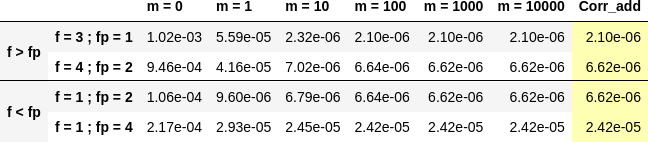
\includegraphics[width=0.8\linewidth]{"corr_ana/tab_errors_fem_circle.png"}
			\captionof{figure}{Errors $||\cdot||_{L^2,rel}$ obtained with different methods on the Circle with standard FEM.}
			\label{tab_errors_fem_circle}
		\end{figure} 
	\end{minipage}
	\begin{minipage}{0.48\linewidth} \qquad 
		\begin{figure}[H]
			\centering
			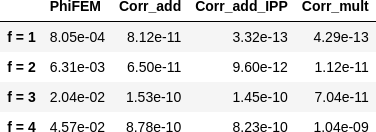
\includegraphics[width=0.8\linewidth]{"corr_ana/tab_errors_phifem_circle.png"}
			\captionof{figure}{Errors $||\cdot||_{L^2,rel}$ obtained with different methods on the Circle with $\phi$-FEM.}
			\label{tab_errors_phifem_circle}
		\end{figure} 
	\end{minipage}
	
	\textbf{Non-homogeneous case :}
	
	We consider here the non-homogeneous problem (i.e. with $\varphi=1$) and seek to test the various correction methods with standard FEM and $\phi$-FEM methods.
	
	\begin{minipage}{0.48\linewidth}
		\begin{figure}[H]
			\centering
			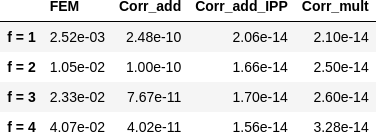
\includegraphics[width=0.8\linewidth]{"corr_ana/tab_errors_fem_circle_nh.png"}
			\captionof{figure}{Errors $||\cdot||_{L^2,rel}$ obtained with different methods on the Circle with standard FEM.}
			\label{tab_errors_fem_circle_nh}
		\end{figure} 
	\end{minipage}
	\begin{minipage}{0.48\linewidth} \qquad 
		\begin{figure}[H]
			\centering
			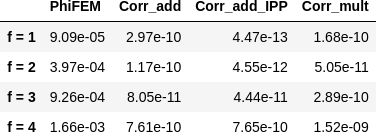
\includegraphics[width=0.8\linewidth]{"corr_ana/tab_errors_phifem_circle_nh.png"}
			\captionof{figure}{Errors $||\cdot||_{L^2,rel}$ obtained with different methods on the Circle with $\phi$-FEM.}
			\label{tab_errors_phifem_circle_nh}
		\end{figure} 
	\end{minipage}
	
	\item \textbf{Results on the Square :}
	
	We consider here the Square problem with the solution defined in Section \ref{Corr.pb.square.1}.
	
	\textbf{Homogeneous case :}
	
	We consider here the homogeneous problem (i.e. with $\varphi=0$) and seek to test the various correction methods with standard FEM and $\phi$-FEM methods.
	
	\begin{minipage}{0.48\linewidth}
		\begin{figure}[H]
			\centering
			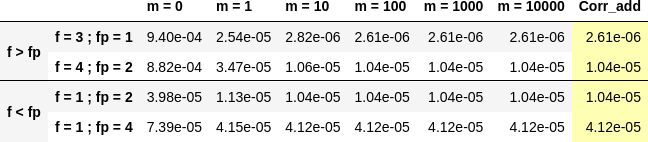
\includegraphics[width=0.8\linewidth]{"corr_ana/tab_errors_fem_square.png"}
			\captionof{figure}{Errors $||\cdot||_{L^2,rel}$ obtained with different methods on the Square with standard FEM.}
			\label{tab_errors_fem_square}
		\end{figure} 
	\end{minipage}
	\begin{minipage}{0.48\linewidth} \qquad 
		\begin{figure}[H]
			\centering
			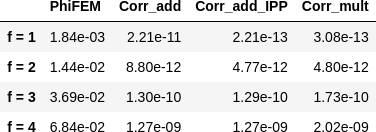
\includegraphics[width=0.8\linewidth]{"corr_ana/tab_errors_phifem_square.png"}
			\captionof{figure}{Errors $||\cdot||_{L^2,rel}$ obtained with different methods on the Square with $\phi$-FEM.}
			\label{tab_errors_phifem_square}
		\end{figure} 
	\end{minipage}
	
	\textbf{Non-homogeneous case :}
	
	We consider here the non-homogeneous problem (i.e. with $\varphi=1$) and seek to test the various correction methods with standard FEM and $\phi$-FEM methods.
	
	\begin{minipage}{0.48\linewidth}
		\begin{figure}[H]
			\centering
			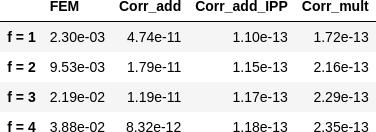
\includegraphics[width=0.8\linewidth]{"corr_ana/tab_errors_fem_square_nh.png"}
			\captionof{figure}{Errors $||\cdot||_{L^2,rel}$ obtained with different methods on the Square with standard FEM.}
			\label{tab_errors_fem_square_nh}
		\end{figure} 
	\end{minipage}
	\begin{minipage}{0.48\linewidth} \qquad 
		\begin{figure}[H]
			\centering
			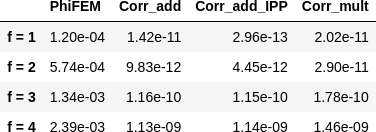
\includegraphics[width=0.8\linewidth]{"corr_ana/tab_errors_phifem_square_nh.png"}
			\captionof{figure}{Errors $||\cdot||_{L^2,rel}$ obtained with different methods on the Square with $\phi$-FEM.}
			\label{tab_errors_phifem_square_nh}
		\end{figure} 
	\end{minipage}
\end{enumerate}

It would therefore seem that the various correction methods work in the different cases considered.

\subsubsection{Correction on disturbed solution} \label{Corr.results.disturbed}
\graphicspath{{images/corr/corr_pert}}

Now, let's consider a deliberately disturbed solution. The purpose of this step is to check that the correction solvers also work with a solution that is very close to the real solution, but not exact. In this section, we will consider a manually disturbed solution, i.e. the exact solution to which we've added a small, analytically known perturbation.

As explained above, we begin by considering $\tilde{\phi}$ as a manually perturbed solution defined by
\begin{equation*}
	\tilde{\phi}(x,y)=u_{ex}(x,y)+\epsilon P(x,y)
\end{equation*}
where $u_{ex}$ defines the exact solution to the problem, $P$ the perturbation applied to it and $\epsilon$ is a real number that allows the amplitude of the perturbation to be easily increased or decreased. 

\begin{Rem}
	Notice that by taking $\epsilon=0$, we return to the case of correction on an exact solution presented in Section \ref{Corr.results.ana}. Recall the relative errors obtained by standard FEM and $\phi$-FEM on the circle and on the square for frequencies $f\in\{1,2,3,4\}$ for the homogeneous  (Figure \ref{norms}) and non-homogeneous problem  (Figure \ref{norms_nh}).
	
	\begin{minipage}{0.48\linewidth}
		\begin{figure}[H]
			\centering
			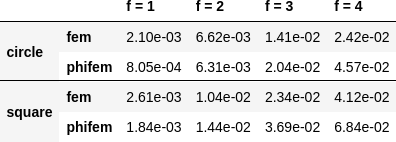
\includegraphics[width=0.8\linewidth]{"corr_pert/norms.png"}
			\captionof{figure}{Table summarizing the errors obtained by standard FEM and $\phi$-FEM on the circle and the square (homogeneous case).}
			\label{norms}
		\end{figure} 
	\end{minipage}
	\begin{minipage}{0.48\linewidth}
		\begin{figure}[H]
			\centering
			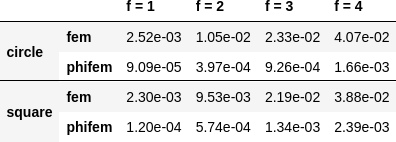
\includegraphics[width=0.8\linewidth]{"corr_pert/norms_nh.png"}
			\captionof{figure}{Table summarizing the errors obtained by standard FEM and $\phi$-FEM on the circle and the square (non-homogeneous case).}
			\label{norms_nh}
		\end{figure} 
	\end{minipage}
\end{Rem}

In our case, we will choose to consider $P$ as being of the same form as our exact solution (defined with different parameters), but we could very well consider a completely different perturbation. 

\begin{Rem}
	Note that the shape of the perturbation has a huge influence on the accuracy of the solvers, and that the difficulty lies in the following cases where its expression is not explicitly known (as in the case of $\phi$-FEM in Section \ref{Corr.results.phifem} or FNO in Section \ref{Corr.results.FNO}).
\end{Rem}

In the case of Circle geometry where we consider the problem \ref{Corr.pb.circle.1}, the perturbation will be defined by
\begin{equation*}
	P(x,y)=S_p\times\sin\left(8\pi f_p\left((x-0.5)^2+(y-0.5)^2\right)+\varphi_p\right)
\end{equation*}
where $S_p\in[0,1]$ is the amplitude of the signal, $f_p\in\mathbb{N}$ can be associated with the "frequency" of the signal and $\varphi_p\in[0,1]$ the phase at the origin.

In the case of Square geometry where we consider the problem \ref{Corr.pb.square.1}, the perturbation will be defined by
\begin{equation*}
	P(x,y)=S_p\times\sin\left(2\pi f_px+\varphi_p\right)\times\sin\left(2\pi f_py+\varphi_p\right)
\end{equation*}
where $S_p\in[0,1]$ is the amplitude of the signal, $f_p\in\mathbb{N}$ can be associated with the "frequency" of the signal and $\varphi_p\in[0,1]$ the phase at the origin.

\begin{Rem}
	Note that for the boundary conditions of the solution to be satisfied, i.e. for $\tilde{\phi}=u_{ex}$ on $\Gamma$, it is essential that $P=0$ on $\Gamma$. In the case of both circle and square, we will then take $\varphi_p=0$.
\end{Rem}

\paragraph{Results with differents $\epsilon$} \label{Corr.results.disturbed.eps} 

\textbf{Results on the homogeneous case :}

First, we consider the homogeneous case (i.e. with $\varphi=0$). The aim is to test correction by addition (without IPP) and correction by multiplication by varying the amplitude of the perturbation (in other words, by varying $\epsilon$). We'll consider the case of the circle and the square for standard FEM and $\phi$-FEM methods, and we'll try to separate the cases according to the frequencies considered. In other words, for $f,f_p\in\{1,2,3,4\}$, we're interested in the following three cases. The first is the case where the solution frequency is greater than the perturbation frequency ($f>f_p$), i.e. a highly variable solution and a less variable perturbation. The second is where the solution and perturbation frequencies are equal ($f=f_p$), i.e. the solution and perturbation have the same variability. The last category covers cases where the perturbation is "nastier" than the solution, i.e. it has a higher frequency than the solution ($f<f_p$).

\begin{enumerate}[label=\textbullet]
	\item \textbf{Results on the Circle :}
	
	We consider here the Circle problem with the solution defined in Section \ref{Corr.pb.circle.1}. Here, we consider correction by adding (without IPP) with standard FEM (Figure \ref{corr_pert_circle_fem_add}) and with $\phi$-FEM (Figure \ref{corr_pert_circle_phifem_add}).
	
	\begin{minipage}{0.48\linewidth}
		\begin{figure}[H]
			\centering
			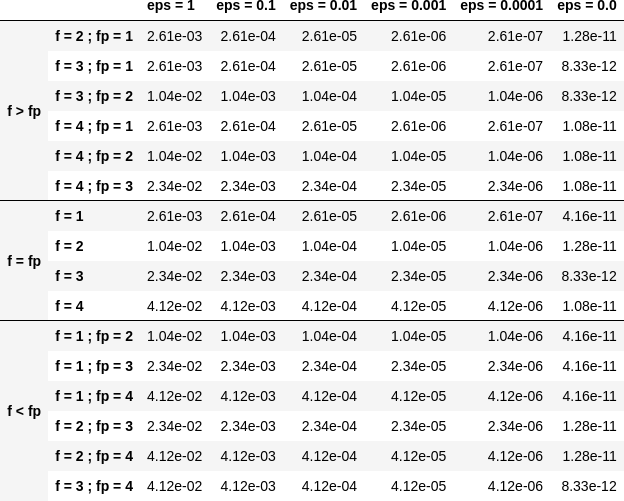
\includegraphics[width=\linewidth]{"corr_pert/corr_pert_circle_fem_add.png"}
			\captionof{figure}{Correction by adding on the Circle with standard FEM.}
			\label{corr_pert_circle_fem_add}
		\end{figure} 
	\end{minipage}
	\begin{minipage}{0.48\linewidth}
		\begin{figure}[H]
			\centering
			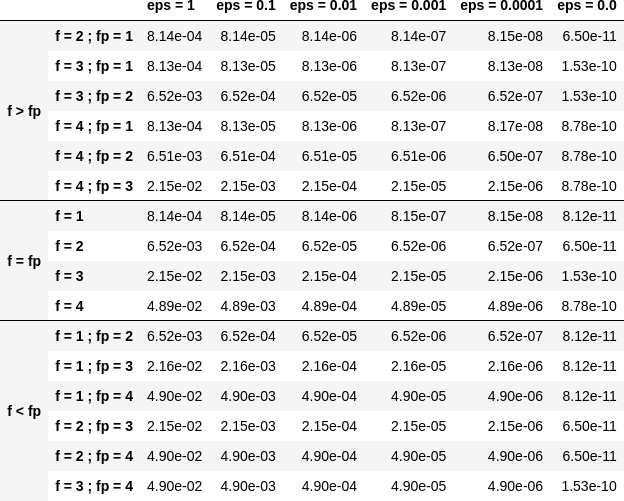
\includegraphics[width=\linewidth]{"corr_pert/corr_pert_circle_phifem_add.png"}
			\captionof{figure}{Correction by adding on the Circle with $\phi$-FEM.}
			\label{corr_pert_circle_phifem_add}
		\end{figure} 
	\end{minipage}
	
	Then, we consider correction by multiplying with standard FEM (Figure \ref{corr_pert_circle_fem_mult}) and with $\phi$-FEM (Figure \ref{corr_pert_circle_phifem_mult}).
	
	\begin{minipage}{0.48\linewidth}
		\begin{figure}[H]
			\centering
			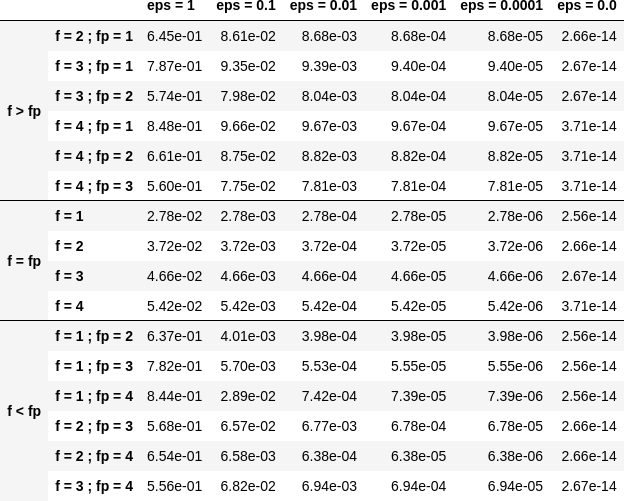
\includegraphics[width=\linewidth]{"corr_pert/corr_pert_circle_fem_mult.png"}
			\captionof{figure}{Correction by multiplying on the Circle with standard FEM.}
			\label{corr_pert_circle_fem_mult}
		\end{figure} 
	\end{minipage}
	\begin{minipage}{0.48\linewidth}
		\begin{figure}[H]
			\centering
			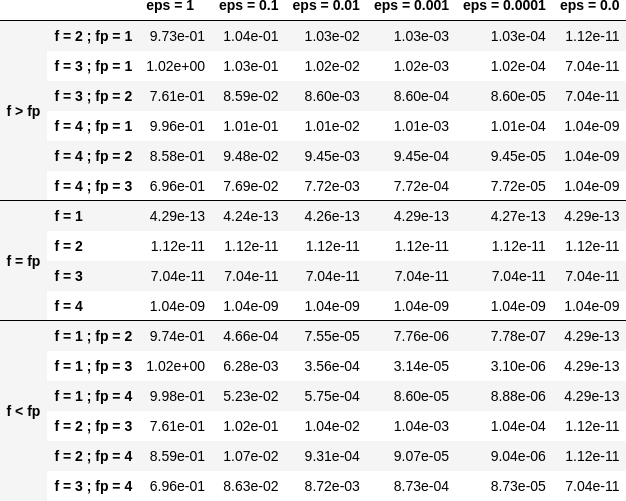
\includegraphics[width=\linewidth]{"corr_pert/corr_pert_circle_phifem_mult.png"}
			\captionof{figure}{Correction by multiplying on the Circle with $\phi$-FEM.}
			\label{corr_pert_circle_phifem_mult}
		\end{figure} 
	\end{minipage}
	
	\item \textbf{Results on the Square :}
	
	We consider here the Square problem with the solution defined in Section \ref{Corr.pb.square.1}. Here, we consider correction by adding (without IPP) with standard FEM (Figure \ref{corr_pert_square_fem_add}) and with $\phi$-FEM (Figure \ref{corr_pert_square_phifem_add}).
	
	\begin{minipage}{0.48\linewidth}
		\begin{figure}[H]
			\centering
			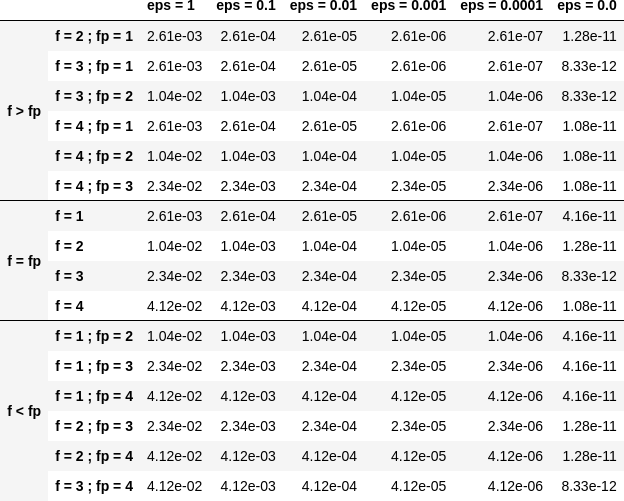
\includegraphics[width=\linewidth]{"corr_pert/corr_pert_square_fem_add.png"}
			\captionof{figure}{Correction by adding on the Square with standard FEM.}
			\label{corr_pert_square_fem_add}
		\end{figure} 
	\end{minipage}
	\begin{minipage}{0.48\linewidth}
		\begin{figure}[H]
			\centering
			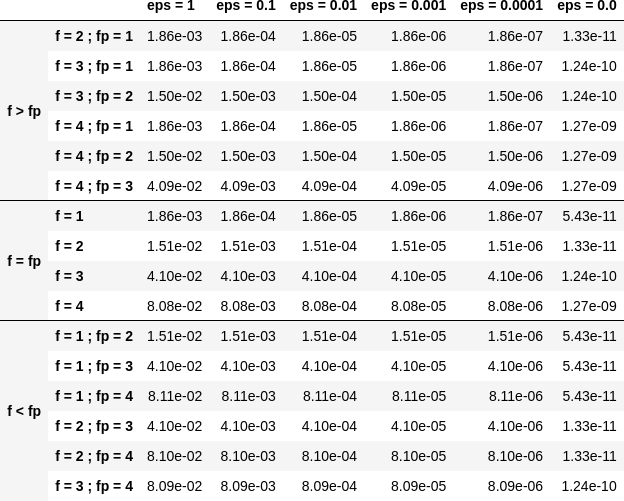
\includegraphics[width=\linewidth]{"corr_pert/corr_pert_square_phifem_add.png"}
			\captionof{figure}{Correction by adding on the Square with $\phi$-FEM.}
			\label{corr_pert_square_phifem_add}
		\end{figure} 
	\end{minipage}
	
	Then, we consider correction by multiplying with standard FEM (Figure \ref{corr_pert_square_fem_mult}) and with $\phi$-FEM (Figure \ref{corr_pert_square_phifem_mult}).
	
	\begin{minipage}{0.48\linewidth}
		\begin{figure}[H]
			\centering
			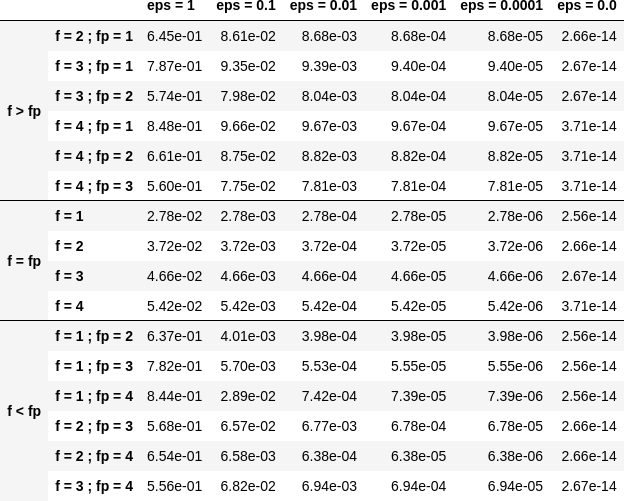
\includegraphics[width=\linewidth]{"corr_pert/corr_pert_square_fem_mult.png"}
			\captionof{figure}{Correction by multiplying on the Square with standard FEM.}
			\label{corr_pert_square_fem_mult}
		\end{figure} 
	\end{minipage}
	\begin{minipage}{0.48\linewidth}
		\begin{figure}[H]
			\centering
			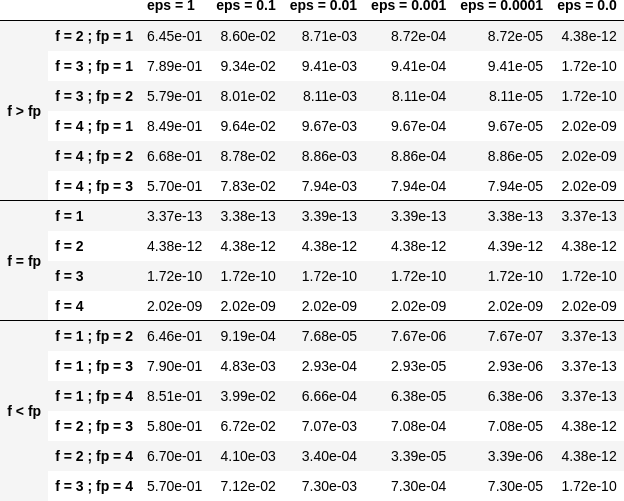
\includegraphics[width=\linewidth]{"corr_pert/corr_pert_square_phifem_mult.png"}
			\captionof{figure}{Correction by multiplying on the Square with $\phi$-FEM.}
			\label{corr_pert_square_phifem_mult}
		\end{figure} 
	\end{minipage}
\end{enumerate}

It would therefore seem that, overall, the smaller the perturbation applied (i.e. the smaller the $\epsilon$), the more efficient the addition and multiplication correction solvers are in terms of accuracy. However, we would like to make a few comments on the results obtained:
\begin{itemize}
	\item First of all, it would appear that, as with the standard FEM and $\phi$-FEM solvers without correction, the more the solution varies (i.e. the larger $f$), the greater the error. This is a fairly intuitive result, since the more the solution varies, the more points are needed to approximate it.
	\item It would also seem that for $\epsilon=1$ (i.e. a large perturbation), this parameter has a greater impact on the multiplicative corrector than on the additive corrector. We explained earlier the benefits of elevating the problem, which could be beneficial here. Results on elevation will be presented in the Section \ref{Corr.results.disturbed.reh}.
	\item In view of the results obtained here, it would also appear that, overall, correction by addition is more effective than correction by multiplication. Moreover, correction by addition has more advantages than correction by multiplication. In particular, if the solution cancels out on the domain, correction by multiplication will require elevating the problem sufficiently so that it no longer cancels out, unlike correction by addition.
	\item An interesting result can also be observed. Indeed, it seems that in the case where $f=f_p$, the multiplication correction with $\phi$-FEM seems to approach the solution almost perfectly for all $\epsilon$ considered.
	In fact, in the homogeneous case, for $f=f_p$ the perturbation is identical to the solution (i.e. $P=u_{ex}$) and so the solution injected into the correction solvers is of the form
	\begin{equation*}
		\tilde{\phi}=u_{ex}+\epsilon P=(1+\epsilon)u_{ex}
	\end{equation*}
	In the case of correction by multiplication, we have $\tilde{u}=\tilde{\phi}C$. So for $\tilde{u}=u_{ex}$, we must have
	\begin{equation*}
		\tilde{\phi}C=u_{ex} \quad \iff \quad (1+\epsilon)u_{ex}C=u_{ex}
	\end{equation*}
	So if the solution does not cancel out on $\Omega$, we must have
	\begin{equation*}
		C=\frac{1}{1+\epsilon} \quad \text{on } \Omega
	\end{equation*}
	By imposing $C=\frac{1}{1+\epsilon}$ on $\Gamma$ for FEM instead of $C=1$, we should get closer to the $\phi$-FEM results obtained. We can see in Figure \ref{norms_circle_f_eq_fp} and Figure \ref{norms_square_f_eq_fp} that we obtain the expected results for FEM by changing the boundary condition $C=1$ to $C=\frac{1}{1+\epsilon}$.
	
	\begin{minipage}{0.48\linewidth}
		\begin{figure}[H]
			\centering
			\includegraphics[width=\linewidth]{"norms_circle_f_eq_fp.png"}
			\captionof{figure}{Results by changing FEM boundary conditions on the circle.}
			\label{norms_circle_f_eq_fp}
		\end{figure} 
	\end{minipage}
	\begin{minipage}{0.48\linewidth}
		\begin{figure}[H]
			\centering
			\includegraphics[width=\linewidth]{"norms_square_f_eq_fp.png"}
			\captionof{figure}{Results by changing FEM boundary conditions on the square.}
			\label{norms_square_f_eq_fp}
		\end{figure} 
	\end{minipage}
	\begin{Rem}
		It should be noted, however, that in practice, for example in the case where $\tilde{\phi}$ is a $\phi$-FEM solution or an FNO output, this case is not very realistic. There's no reason to expect the form of the perturbation created by the $\phi$-FEM solver or by the FNO to be exactly identical to the solution under consideration.
	\end{Rem}
\end{itemize}

\textbf{Results on the non-homogeneous case :}

Then, we consider the non-homogeneous case (i.e. with $\varphi=1$). The aim here is the same as in the homogeneous case, test correction by addition (without IPP) and correction by multiplication by varying the amplitude of the perturbation (in other words, by varying $\epsilon$). We'll consider the case of the circle and the square for standard FEM and $\phi$-FEM methods, and we'll try to separate the cases according to the frequencies considered. In other words, for $f,f_p\in\{1,2,3,4\}$, we're interested in the following three cases. The first is the case where the solution frequency is greater than the perturbation frequency ($f>f_p$), i.e. a highly variable solution and a less variable perturbation. The second is where the solution and perturbation frequencies are equal ($f=f_p$), i.e. the solution and perturbation have the same variability. The last category covers cases where the perturbation is "nastier" than the solution, i.e. it has a higher frequency than the solution ($f<f_p$).

\begin{enumerate}[label=\textbullet]
	\item \textbf{Results on the Circle :}
	
	We consider here the Circle problem with the solution defined in Section \ref{Corr.pb.circle.1}. Here, we consider correction by adding (without IPP) with standard FEM (Figure \ref{corr_pert_circle_fem_nh_add}) and with $\phi$-FEM (Figure \ref{corr_pert_circle_phifem_nh_add}).
	
	\begin{minipage}{0.48\linewidth}
		\begin{figure}[H]
			\centering
			\includegraphics[width=\linewidth]{"corr_pert_circle_fem_nh_add.png"}
			\captionof{figure}{Correction by adding on the Circle with standard FEM.}
			\label{corr_pert_circle_fem_nh_add}
		\end{figure} 
	\end{minipage}
	\begin{minipage}{0.48\linewidth}
		\begin{figure}[H]
			\centering
			\includegraphics[width=\linewidth]{"corr_pert_circle_phifem_nh_add.png"}
			\captionof{figure}{Correction by adding on the Circle with $\phi$-FEM.}
			\label{corr_pert_circle_phifem_nh_add}
		\end{figure} 
	\end{minipage}
	
	Then, we consider correction by multiplying with standard FEM (Figure \ref{corr_pert_circle_fem_nh_mult}) and with $\phi$-FEM (Figure \ref{corr_pert_circle_phifem_nh_mult}).
	
	\begin{minipage}{0.48\linewidth}
		\begin{figure}[H]
			\centering
			\includegraphics[width=\linewidth]{"corr_pert_circle_fem_nh_mult.png"}
			\captionof{figure}{Correction by multiplying on the Circle with standard FEM.}
			\label{corr_pert_circle_fem_nh_mult}
		\end{figure} 
	\end{minipage}
	\begin{minipage}{0.48\linewidth}
		\begin{figure}[H]
			\centering
			\includegraphics[width=\linewidth]{"corr_pert_circle_phifem_nh_mult.png"}
			\captionof{figure}{Correction by multiplying on the Circle with $\phi$-FEM.}
			\label{corr_pert_circle_phifem_nh_mult}
		\end{figure} 
	\end{minipage}
	
	\item \textbf{Results on the Square :}
	
	We consider here the Square problem with the solution defined in Section \ref{Corr.pb.square.1}. Here, we consider correction by adding (without IPP) with standard FEM (Figure \ref{corr_pert_square_fem_nh_add}) and with $\phi$-FEM (Figure \ref{corr_pert_square_phifem_nh_add}).
	
	\begin{minipage}{0.48\linewidth}
		\begin{figure}[H]
			\centering
			\includegraphics[width=\linewidth]{"corr_pert_square_fem_nh_add.png"}
			\captionof{figure}{Correction by adding on the Square with standard FEM.}
			\label{corr_pert_square_fem_nh_add}
		\end{figure} 
	\end{minipage}
	\begin{minipage}{0.48\linewidth}
		\begin{figure}[H]
			\centering
			\includegraphics[width=\linewidth]{"corr_pert_square_phifem_nh_add.png"}
			\captionof{figure}{Correction by adding on the Square with $\phi$-FEM.}
			\label{corr_pert_square_phifem_nh_add}
		\end{figure} 
	\end{minipage}
	
	Then, we consider correction by multiplying with standard FEM (Figure \ref{corr_pert_square_fem_nh_mult}) and with $\phi$-FEM (Figure \ref{corr_pert_square_phifem_nh_mult}).
	
	\begin{minipage}{0.48\linewidth}
		\begin{figure}[H]
			\centering
			\includegraphics[width=\linewidth]{"corr_pert_square_fem_nh_mult.png"}
			\captionof{figure}{Correction by multiplying on the Square with standard FEM.}
			\label{corr_pert_square_fem_nh_mult}
		\end{figure} 
	\end{minipage}
	\begin{minipage}{0.48\linewidth}
		\begin{figure}[H]
			\centering
			\includegraphics[width=\linewidth]{"corr_pert_square_phifem_nh_mult.png"}
			\captionof{figure}{Correction by multiplying on the Square with $\phi$-FEM.}
			\label{corr_pert_square_phifem_nh_mult}
		\end{figure} 
	\end{minipage}
\end{enumerate}

In view of the results obtained, it would appear that the conclusions are the same as for the homogeneous case. Except for the case where $f=f_p$, because in the case where the solution is non-homogeneous (i.e. $u_{ex}=g$ on $\Gamma$), the perturbation $P$ is no longer equal to the solution $u_{ex}$ because $P=0$ on $\Gamma$.

\paragraph{Results on the elevated problem} \label{Corr.results.disturbed.reh} 

\trad{On testera que en homogène ici}

\modif{Résultats sur le rehaussement + montrer que quand la solution s'annule c'est bcp mieux}

\subsubsection{Correction on $\phi$-FEM solution} \label{Corr.results.phifem}

\modif{Then we'll look at correcting a disturbed solution for which we don't know the form of the perturbation. A $\phi$-FEM solution can be considered for injection into correction solvers.}

\subsubsection{Correction with FNO} \label{Corr.results.FNO}

\subsubsection{Correction with other networks} \label{Corr.results.neural_net}

\paragraph{Multiperceptron} \label{Corr.results.neural_net.multiperceptron}

\paragraph{PINNs} \label{Corr.results.neural_net.PINNs}
	
	\newpage
	\section{Conclusion}

The main objective of the internship was to combine finite element methods and machine learning in order to solve the Poisson problem with boundary Dirichlet condition. More precisely, we wanted to train an FNO to predict the solutions of a PDE for a given family of problems and apply a correction to them using finite element solvers with the aim of improving the accuracy of the solution. 

We have considered 2 types of solution correction methods, the first is an addition correction method and the second is a multiplication correction method, which have been treated by the FEM and $\phi$-FEM methods. We have chosen here the case of fairly simple solutions on very simple and fixed geometries, which have enabled us to obtain numerical results on analytical solutions. These test cases have enabled us to confirm that the correction methods considered are functional, and have also confirmed some of the theoretical results obtained. These initial test cases also enabled us to identify some of the limitations of these correction methods, particularly in terms of the degrees of the chosen spaces.  

 We were then able to apply these various correction methods to the predictions made by the FNO, and it turned out that the results were not satisfactory. As a result, we began to look for methods to increase the degree of the solution in order to bring us back to the results obtained in the analytical cases. The first idea was to decompose the FNO output into a series of polynomials ( notably Legendre polynomials) in order to evaluate the solution at any point in our domain and thus consider the high-degree solution.

As the results were inconclusive, we turned to neural networks. Putting the FNO to one side, we set out to build a neural network model capable of predicting a solution at any point in the domain. We began by considering an MLP network, whose lack of learning on derivatives proved problematic. We then moved on to PINNs, which, by learning the solution, also learn its derivatives, enabling us to reduce the error made by conventional methods (FEM and $\phi$-FEM) by a factor of around 100 (in the case of correction by addition). 

Following on from what has already been done, we could then try adding PINNs to the output of the FNO, in other words, adding a layer output that would replace the decomposition into a series of polynomials and enable us to have the solution at any point in the domain. We could also carry out some documentation work to find more suitable models than the FNO. Finally, we could consider more complex and time-varying geometries (such as 3D organ geometries).
	
	\newpage
	\section*{Bibliography}
	\addcontentsline{toc}{section}{Bibliography}
		
	\printbibliography
	
\end{document}